\documentclass[a4paper, 12pt]{report}

%====================== PACKAGES ======================

\usepackage[french]{babel}
\usepackage[utf8x]{inputenc}
%pour gérer les positionnement d'images
\usepackage{float}
\usepackage{amsmath}
\usepackage{graphicx}
\usepackage[colorinlistoftodos]{todonotes}
\usepackage{url}
%pour les informations sur un document compilé en PDF et les liens externes / internes
\usepackage{hyperref}
%pour la mise en page des tableaux
\usepackage{array}
\usepackage{tabularx}
%pour utiliser \floatbarrier
%\usepackage{placeins}
%\usepackage{floatrow}
%espacement entre les lignes
\usepackage{setspace}
%modifier la mise en page de l'abstract
\usepackage{abstract}
%police et mise en page (marges) du document
\usepackage[T1]{fontenc}
\usepackage[top=2cm, bottom=2cm, left=2cm, right=2cm]{geometry}
%Pour les galerie d'images
\usepackage{subfig}
\usepackage{eurosym}
%Pour la mise en page du code
\usepackage{listings}
\usepackage{color}
\definecolor{dkgreen}{rgb}{0,0.6,0}
\definecolor{gray}{rgb}{0.5,0.5,0.5}
\definecolor{mauve}{rgb}{0.58,0,0.82}
\usepackage{dirtree}
\usepackage{underscore}


\lstdefinestyle{tf}{frame=shadowbox,
	rulesepcolor=\color{gray},
	framexleftmargin=5mm,
	aboveskip=3mm,
	belowskip=3mm,
	showstringspaces=false,
	columns=flexible,
	basicstyle={\small\ttfamily},
	numbers=left,
	numberstyle=\tiny,
	breaklines=true,
	tabsize=3
}

\lstset{frame=tb,
	extendedchars=true,
	inputencoding=latin1,
	rulesepcolor=\color{gray},
	framexleftmargin=5mm,
	language=bash,
	aboveskip=3mm,
	belowskip=3mm,
	showstringspaces=false,
	columns=flexible,
	basicstyle={\small\ttfamily},
	numbers=left,
	numberstyle=\tiny,
	keywordstyle=\color{blue},
	stringstyle=\color{mauve},
	breaklines=true,
	tabsize=3,
	literate=%
	{é}{{\'e}}{1}%
	{è}{{\`e}}{1}%
	{à}{{\`a}}{1}%
	{ç}{{\c{c}}}{1}%
	{œ}{{\oe}}{1}%
	{ù}{{\`u}}{1}%
	{É}{{\'E}}{1}%
	{È}{{\`E}}{1}%
	{À}{{\`A}}{1}%
	{Ç}{{\c{C}}}{1}%
	{Œ}{{\OE}}{1}%
	{Ê}{{\^E}}{1}%
	{ê}{{\^e}}{1}%
	{î}{{\^i}}{1}%
	{ô}{{\^o}}{1}%
	{û}{{\^u}}{1}%
	{ä}{{\"{a}}}1
	{ë}{{\"{e}}}1
	{ï}{{\"{i}}}1
	{ö}{{\"{o}}}1
	{ü}{{\"{u}}}1
	{û}{{\^{u}}}1
	{â}{{\^{a}}}1
	{Â}{{\^{A}}}1
	{Î}{{\^{I}}}1
}
%====================== INFORMATION ET REGLES ======================

%rajouter les numérotation pour les \paragraphe et \subparagraphe
\setcounter{secnumdepth}{4}
\setcounter{tocdepth}{4}

\hypersetup{							% Information sur le document
pdfauthor = {Florian HEGELE,
			Yahia KHERZA,
			Olivier MARAVAL,
    		Valentin VIRET-JACQUOT,
    		Manon LAMBLOT},			% Auteurs
pdftitle = {Définition des besoins},			% Titre du document
pdfsubject = {SAE203 - Livrable 1},		% Sujet
pdfkeywords = {Tag1, Tag2, Tag3, ...},	% Mots-clefs
pdfstartview={FitH}}					% ajuste la page à la largueur de l'écran
%pdfcreator = {MikTeX},% Logiciel qui a crée le document
%pdfproducer = {}} % Société avec produit le logiciel

%======================== DEBUT DU DOCUMENT ========================

\begin{document}

\addtocontents{toc}{\protect\thispagestyle{empty}}

%régler l'espacement entre les lignes
\newcommand{\HRule}{\rule{\linewidth}{0.5mm}}

%page de garde
\begin{titlepage}
\begin{center}

% Upper part of the page. The '~' is needed because only works if a paragraph has started.

\includegraphics[width=0.5\textwidth]{./images/InfoLogoQuadriH.png}~\\[1cm]

\textsc{\LARGE SAE 2.03 - BUT INFORMATIQUE - GROUPE 1}\\[1.5cm]

\textsc{\Large }\\[0.5cm]

% Title
\HRule \\[0.4cm]

{\huge \bfseries Dossier de définition des besoins pour l'hébergement de l'application meuuuhble\\[0.4cm] }

\HRule \\[1.5cm]

% Author and supervisor
\begin{minipage}{0.4\textwidth}
\begin{flushleft} \large
\emph{Auteur:}\\
Florian \textsc{Hegele}(\textit{A1})\\
Yahia \textsc{Kherza}(\textit{A1})\\
Olivier \textsc{Maraval}(\textit{A1})\\
Manon \textsc{Lamblot}(\textit{A1})\\
\end{flushleft}
\end{minipage}
\begin{minipage}{0.4\textwidth}
\begin{flushright} \large
\emph{Client:} \\
Michel \textsc{Salomon}\\
\emph{Référent:} \\
Olivier \textsc{Maraval}
\end{flushright}
\end{minipage}

\vfill

% Bottom of the page
{\large \today}

\end{center}
\end{titlepage}

%page blanche
\newpage
~
\thispagestyle{empty}


\pagenumbering{gobble}
\tableofcontents
\thispagestyle{empty}

%ne pas numéroter le sommaire

\newpage

%espacement entre les lignes d'un tableau
\renewcommand{\arraystretch}{1.5}

%====================== INCLUSION DES PARTIES ======================

~
\thispagestyle{empty}


\newpage
\pagenumbering{arabic}

\setcounter{page}{5}


\chapter{Description de l'application développée}

Meuuuhble entend développer un nouveau canal de distribution en investissant dans le
commerce en ligne, ce qui permettra de toucher une clientèle plus large et de faciliter l'expansion à
l'international. La plateforme digitale sera conçue pour offrir une expérience utilisateur intuitive et engageante,
renforçant ainsi la présence en ligne de Meuuuhble et son image de marque. C'est en cela que consistera la boutique en ligne développée pour Meuuuhble.

\section{Description non technique de l'application}

L'application développée est une plateforme de commerce en ligne dédiée à la vente de meubles. Elle permet aux utilisateurs de parcourir un catalogue de meubles, de les ajouter à leur panier, de passer commande, et de laisser des commentaires sur les produits qu'ils ont achetés.\\

Voici les points clés définissant l'application éponyme de l'entreprise Meuuuhble :
\begin{itemize}
	\item \textbf{Achat d'articles :} Le site permettra aux utilisateurs d'acheter des meubles en ligne, avec un processus
	de paiement sécurisé et une interface claire pour faciliter la transaction.
	\item \textbf{Recherche avancée d'articles : }Une fonctionnalité de recherche avec des filtres dynamiques sera
	intégrée, permettant aux clients de trouver facilement des articles selon différents critères tels que la catégorie, le prix, la couleur, le matériau, etc. Les articles pourront se décliner en différentes variantes, offrant ainsi un choix plus large.
	\item \textbf{Commentaires et évaluations :} Les utilisateurs auront la possibilité de commenter et de noter les	articles qu'ils ont achetés, ce qui fournira des retours précieux à la fois pour Meuuuhble et pour les futurs acheteurs.
	\item \textbf{Gestion des adresses d'expédition :} Les clients pourront enregistrer plusieurs adresses d'expédition et sélectionner l'adresse préférée lors du processus de commande, simplifiant ainsi les achats
	répétés.
	\item \textbf{Liste d'envies et historique :} Le site offrira la possibilité de créer une liste d'envies où les clients	pourront sauvegarder leurs articles préférés pour un achat futur. Un historique des derniers articles consultés sera également disponible pour faciliter la reprise du shopping.\\
\end{itemize}


Ces fonctionnalités sont conçues pour améliorer l'expérience client en ligne, augmenter
l'engagement et favoriser la fidélisation. Elles soutiendront également les objectifs commerciaux de
Meuuuhble en augmentant le taux de conversion et en élargissant sa clientèle.

\section{Description technique de l'application}

L'application utilise le framework web Flask pour le backend, écrit en Python. Flask est choisi pour sa simplicité et sa flexibilité, permettant de développer rapidement des applications web avec une structure claire et maintenable. L'architecture logicielle repose sur une séparation entre la logique de présentation (templates HTML) et la logique métier (contrôleurs).

\subsection{Langages de Programmation}
\begin{itemize}
	\item \textbf{Frontend:} \textbf{JavaScript}, \textbf{HTML5}, \textbf{CSS3}
	\item \textbf{Backend:} \textbf{Python 3}, avec \textbf{Flask} comme framework web et \textbf{Jinja} comme moteur de template	
\end{itemize}

\subsection{Bibliothèques et Frameworks}
\begin{itemize}
	\item \textbf{Bootstrap} pour la construction de l'interface utilisateur
	\item \textbf{Flask :} Framework web en Python pour la création d'applications web et notamment les fonctionnalités suivantes :
	\begin{itemize}
		\item \textbf{request :} Permet d'accéder aux données de la requête entrante.
		\item \textbf{render_template : }Utilisé pour rendre des modèles Jinja2 pour générer des pages HTML.
		\item \textbf{redirect :} Redirige l'utilisateur vers une autre URL.
		\item \textbf{url_for} : Génère une URL pour une fonction de vue spécifique.
		\item \textbf{abort :} Arrête le traitement d'une requête et renvoie une réponse d'erreur.
		\item \textbf{flash :} Utilisé pour afficher un message flash à l'utilisateur.
		\item \textbf{session :} Permet de stocker des informations utilisateur entre les requêtes.
		\item \textbf{g :} Objet global qui est utilisé pour stocker des données pendant toute la durée d'une requête.
		\item \textbf{blueprint :} Permet de créer des modules Flask réutilisables et modulaires, regroupant des routes, des vues et d'autres fonctionnalités liées.
	\end{itemize}
	\item \textbf{SQLAlchemy :} Utilisé comme ORM pour faciliter l'interaction avec la base de données.
	\item \textbf{pymysql :} Utilisé pour se connecter à une base de données MySQL et d'exécuter des requêtes SQL en utilisant Python
\end{itemize}

\subsection{Base de Données}
\begin{itemize}
	\item \textbf{mysql} pour le stockage des données relationnelles
\end{itemize}

\subsection{Infrastructure et Déploiement}
\begin{itemize}
	\item \textbf{Git} pour le contrôle de version
	\item \textbf{Python-Anywhere} pour la présentation d'une maquette fonctionnelle au client
\end{itemize}

\subsection{Outils utilisés pour le développement}

\begin{itemize}
	\item \textbf{Visual Studio Code} et \textbf{Pycharm} pour le développement de l'application web.
	\item \textbf{Datagrip} pour assister la gestion de la base de données mysql.
	\item \textbf{Looping} pour l'élaboration du MCD et du MLD.
\end{itemize}

\subsection{Arborescence des Fichiers}

Voici la représentation de l'arborescence des fichiers pour l'application meuuuhble :\\

\dirtree{%
.1 meuuuhble/.
	.2 controllers/.
		.3 \textit{Contient les fichiers python assurant le fonctionnement du site}.
	.2 static/.
		.3 assets/.
			.4 \textit{Contient les scripts js et les feuilles de style css}.
		.3 images/.
			.4 \textit{Contient les photos des produits vendus}.
		.3 images_asset/.
			.4 \textit{Contient les images nécessaire a l'affichage du site}.
	.2 templates/.
		.3 admin/.
			.4 \textit{Contient les templates jinja des pages côté administrateur}.
		.3 auth/.
			.4 \textit{Contient les templates jinja des pages d'authentifications}.
		.3 client/.
			.4 \textit{Contient les templates jinja des pages côté client}.
}

\chapter{Analyse des besoins}

Intro

\section{Besoins fonctionnels}

Après une analyse des besoins fonctionnels du projet, nous avons défini deux sous catégories. D'un côté, les besoins [...], de l'autre, les besoins [...].

\subsection{Sous-partie 1}

Bla

\subsection{Sous-partie 2}

Bla

\newpage

\section{Besoins non-fonctionnels}

Comme précédemment, nous avons choisi de distinguer deux catégories pour les besoins non-fonctionnels. D'une part, nous avons les besoins non-fonctionnels pour les [...], et d'autre part ceux pour [...]. Nous avons aussi pris en compte les contraintes de développement, que nous détaillerons à la fin de cette partie.

\subsection{Sous-partie 1}

Bla\\

Aperçu du rendu souhaité :

\begin{figure}[!h]
\begin{center}
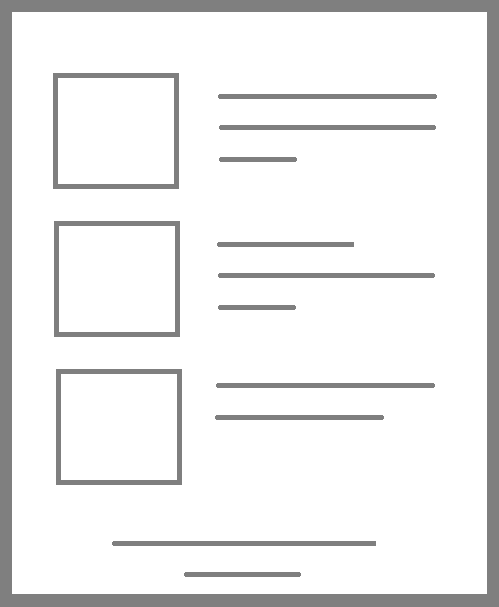
\includegraphics[height=10cm]{besoins/rendu}
\end{center}
\caption{Rendu attendu}
\end{figure}

\subsection{Sous-partie 2}

Bla

\newpage

\section{Développement}

Intro

\subsection{Tâches}

Bla\\


%tableau à taille fixée sur certaines colonnes (param sur la ligne \begin{tabularx}, voir wiki pour plus d'info sur la syntaxe
\begin{figure}[!h]
\begin{center}
\begin{tabularx}{17cm}{|c|p{6cm}|X|}
  \hline
  Priorité & Nom & Raison\\
  \hline
  1 & Tache 1 & Doit être vérifié en premier car sinon [...] \tabularnewline
  2 & Tache 2 & On doit pouvoir [...] \tabularnewline
  3 & Tache 3 & Comme les principales fonctionnalités permettant de tester sont opérationnelles, nous pouvons passer à cette tâche. \tabularnewline
  4 & Tache 4 & Parce que [...] \tabularnewline
  5 & Tache 5 & La tache 5 fait partie des principales [...]. \tabularnewline
  6 & Tache 6 & Dernière fonctionnalité essentielle à mettre en place. \tabularnewline
  7 & Tache 7 & Non-essentiel, mais apporterait un plus au projet. \tabularnewline
  8 & Tache 8 & Non-essentiel, mais apporterait un plus au projet. \tabularnewline
  \hline
\end{tabularx}
\end{center}
\caption{Tableau récapitulatif des tâches}
\end{figure}

\subsection{Tests}

Bla\\

\begin{figure}[!h]
\begin{center}
\begin{tabularx}{17cm}{|p{6cm}|X|}
  \hline
  Fonctionnalité & Test\\
  \hline
  Fonction 1 & Quand [...], vérifier [...]. \tabularnewline
  & Et quand [...], vérifier [...]. \tabularnewline
  Fonction 2 & Vérifier [...]. \tabularnewline
  Fonction 3 & Vérifier [...]. \tabularnewline
  Fonction 4 & Avoir [...]. \tabularnewline
  Fonction 5 & Accéder à [...]. \tabularnewline
   & Vérifier que [...]. \tabularnewline
  Fonction 6 & Accéder à [...]. \tabularnewline
   & Et vérifier [...]. \tabularnewline
  Fonction 7 & Installer [...]. \tabularnewline
   & Vérifier [...]. \tabularnewline
  Fonction 8 & Compter [...]. \tabularnewline
  \hline
\end{tabularx}
\end{center}
\caption{Tableau récapitulatif des tests}
\end{figure}

\newpage

%récupérer les citation avec "/footnotemark"
\nocite{*}



\end{document}